% Options for packages loaded elsewhere
\PassOptionsToPackage{unicode}{hyperref}
\PassOptionsToPackage{hyphens}{url}
\documentclass[
]{article}
\usepackage{xcolor}
\usepackage[margin=1in]{geometry}
\usepackage{amsmath,amssymb}
\setcounter{secnumdepth}{-\maxdimen} % remove section numbering
\usepackage{iftex}
\ifPDFTeX
  \usepackage[T1]{fontenc}
  \usepackage[utf8]{inputenc}
  \usepackage{textcomp} % provide euro and other symbols
\else % if luatex or xetex
  \usepackage{unicode-math} % this also loads fontspec
  \defaultfontfeatures{Scale=MatchLowercase}
  \defaultfontfeatures[\rmfamily]{Ligatures=TeX,Scale=1}
\fi
\usepackage{lmodern}
\ifPDFTeX\else
  % xetex/luatex font selection
\fi
% Use upquote if available, for straight quotes in verbatim environments
\IfFileExists{upquote.sty}{\usepackage{upquote}}{}
\IfFileExists{microtype.sty}{% use microtype if available
  \usepackage[]{microtype}
  \UseMicrotypeSet[protrusion]{basicmath} % disable protrusion for tt fonts
}{}
\makeatletter
\@ifundefined{KOMAClassName}{% if non-KOMA class
  \IfFileExists{parskip.sty}{%
    \usepackage{parskip}
  }{% else
    \setlength{\parindent}{0pt}
    \setlength{\parskip}{6pt plus 2pt minus 1pt}}
}{% if KOMA class
  \KOMAoptions{parskip=half}}
\makeatother
\usepackage{graphicx}
\makeatletter
\newsavebox\pandoc@box
\newcommand*\pandocbounded[1]{% scales image to fit in text height/width
  \sbox\pandoc@box{#1}%
  \Gscale@div\@tempa{\textheight}{\dimexpr\ht\pandoc@box+\dp\pandoc@box\relax}%
  \Gscale@div\@tempb{\linewidth}{\wd\pandoc@box}%
  \ifdim\@tempb\p@<\@tempa\p@\let\@tempa\@tempb\fi% select the smaller of both
  \ifdim\@tempa\p@<\p@\scalebox{\@tempa}{\usebox\pandoc@box}%
  \else\usebox{\pandoc@box}%
  \fi%
}
% Set default figure placement to htbp
\def\fps@figure{htbp}
\makeatother
\setlength{\emergencystretch}{3em} % prevent overfull lines
\providecommand{\tightlist}{%
  \setlength{\itemsep}{0pt}\setlength{\parskip}{0pt}}
\usepackage{bookmark}
\IfFileExists{xurl.sty}{\usepackage{xurl}}{} % add URL line breaks if available
\urlstyle{same}
\hypersetup{
  pdftitle={Clustering Report},
  pdfauthor={Carson Mowrer},
  hidelinks,
  pdfcreator={LaTeX via pandoc}}

\title{Clustering Report}
\author{Carson Mowrer}
\date{2025-10-24}

\begin{document}
\maketitle

\section{Task 1: K-Means Clustering on Hypercube
Data}\label{task-1-k-means-clustering-on-hypercube-data}

In this task, I generated data from clusters centered at the positive
corners of an \(n\)-dimensional hypercube. Each corner represented a
separate cluster. The goal was to determine how close the clusters could
be moved toward the origin before k-means clustering and the
\texttt{clusGap()} function used for determining the optimal number of
clusters failed to detect the true number of clusters.

For each dimension \(n = 2, 3, 4, 5, 6\), I gradually decreased the side
length of the hypercube and evaluated whether \texttt{clusGap()}
selected the correct number of clusters. The results showed a clear
inflection point: when the side length was large enough, the algorithm
performed well, but below a certain threshold, the clusters became too
close for k-means to reliably distinguish.

Specifically:

\begin{itemize}
\tightlist
\item
  For \(n = 6\), the correct number of clusters was identified when the
  side length ≥ 4.
\item
  For \(n = 5\), the inflection occurred at 3.75.
\item
  For \(n = 4\), at 3.5.
\item
  For \(n = 3\), at 2.5.
\item
  For \(n = 2\), at 2.
\end{itemize}

This pattern reflects that as the dimensionality increases, clusters
must be spaced further apart in Euclidean distance for k-means to detect
them as distinct.

The figure below summarizes these findings.

\begin{figure}
\centering
\pandocbounded{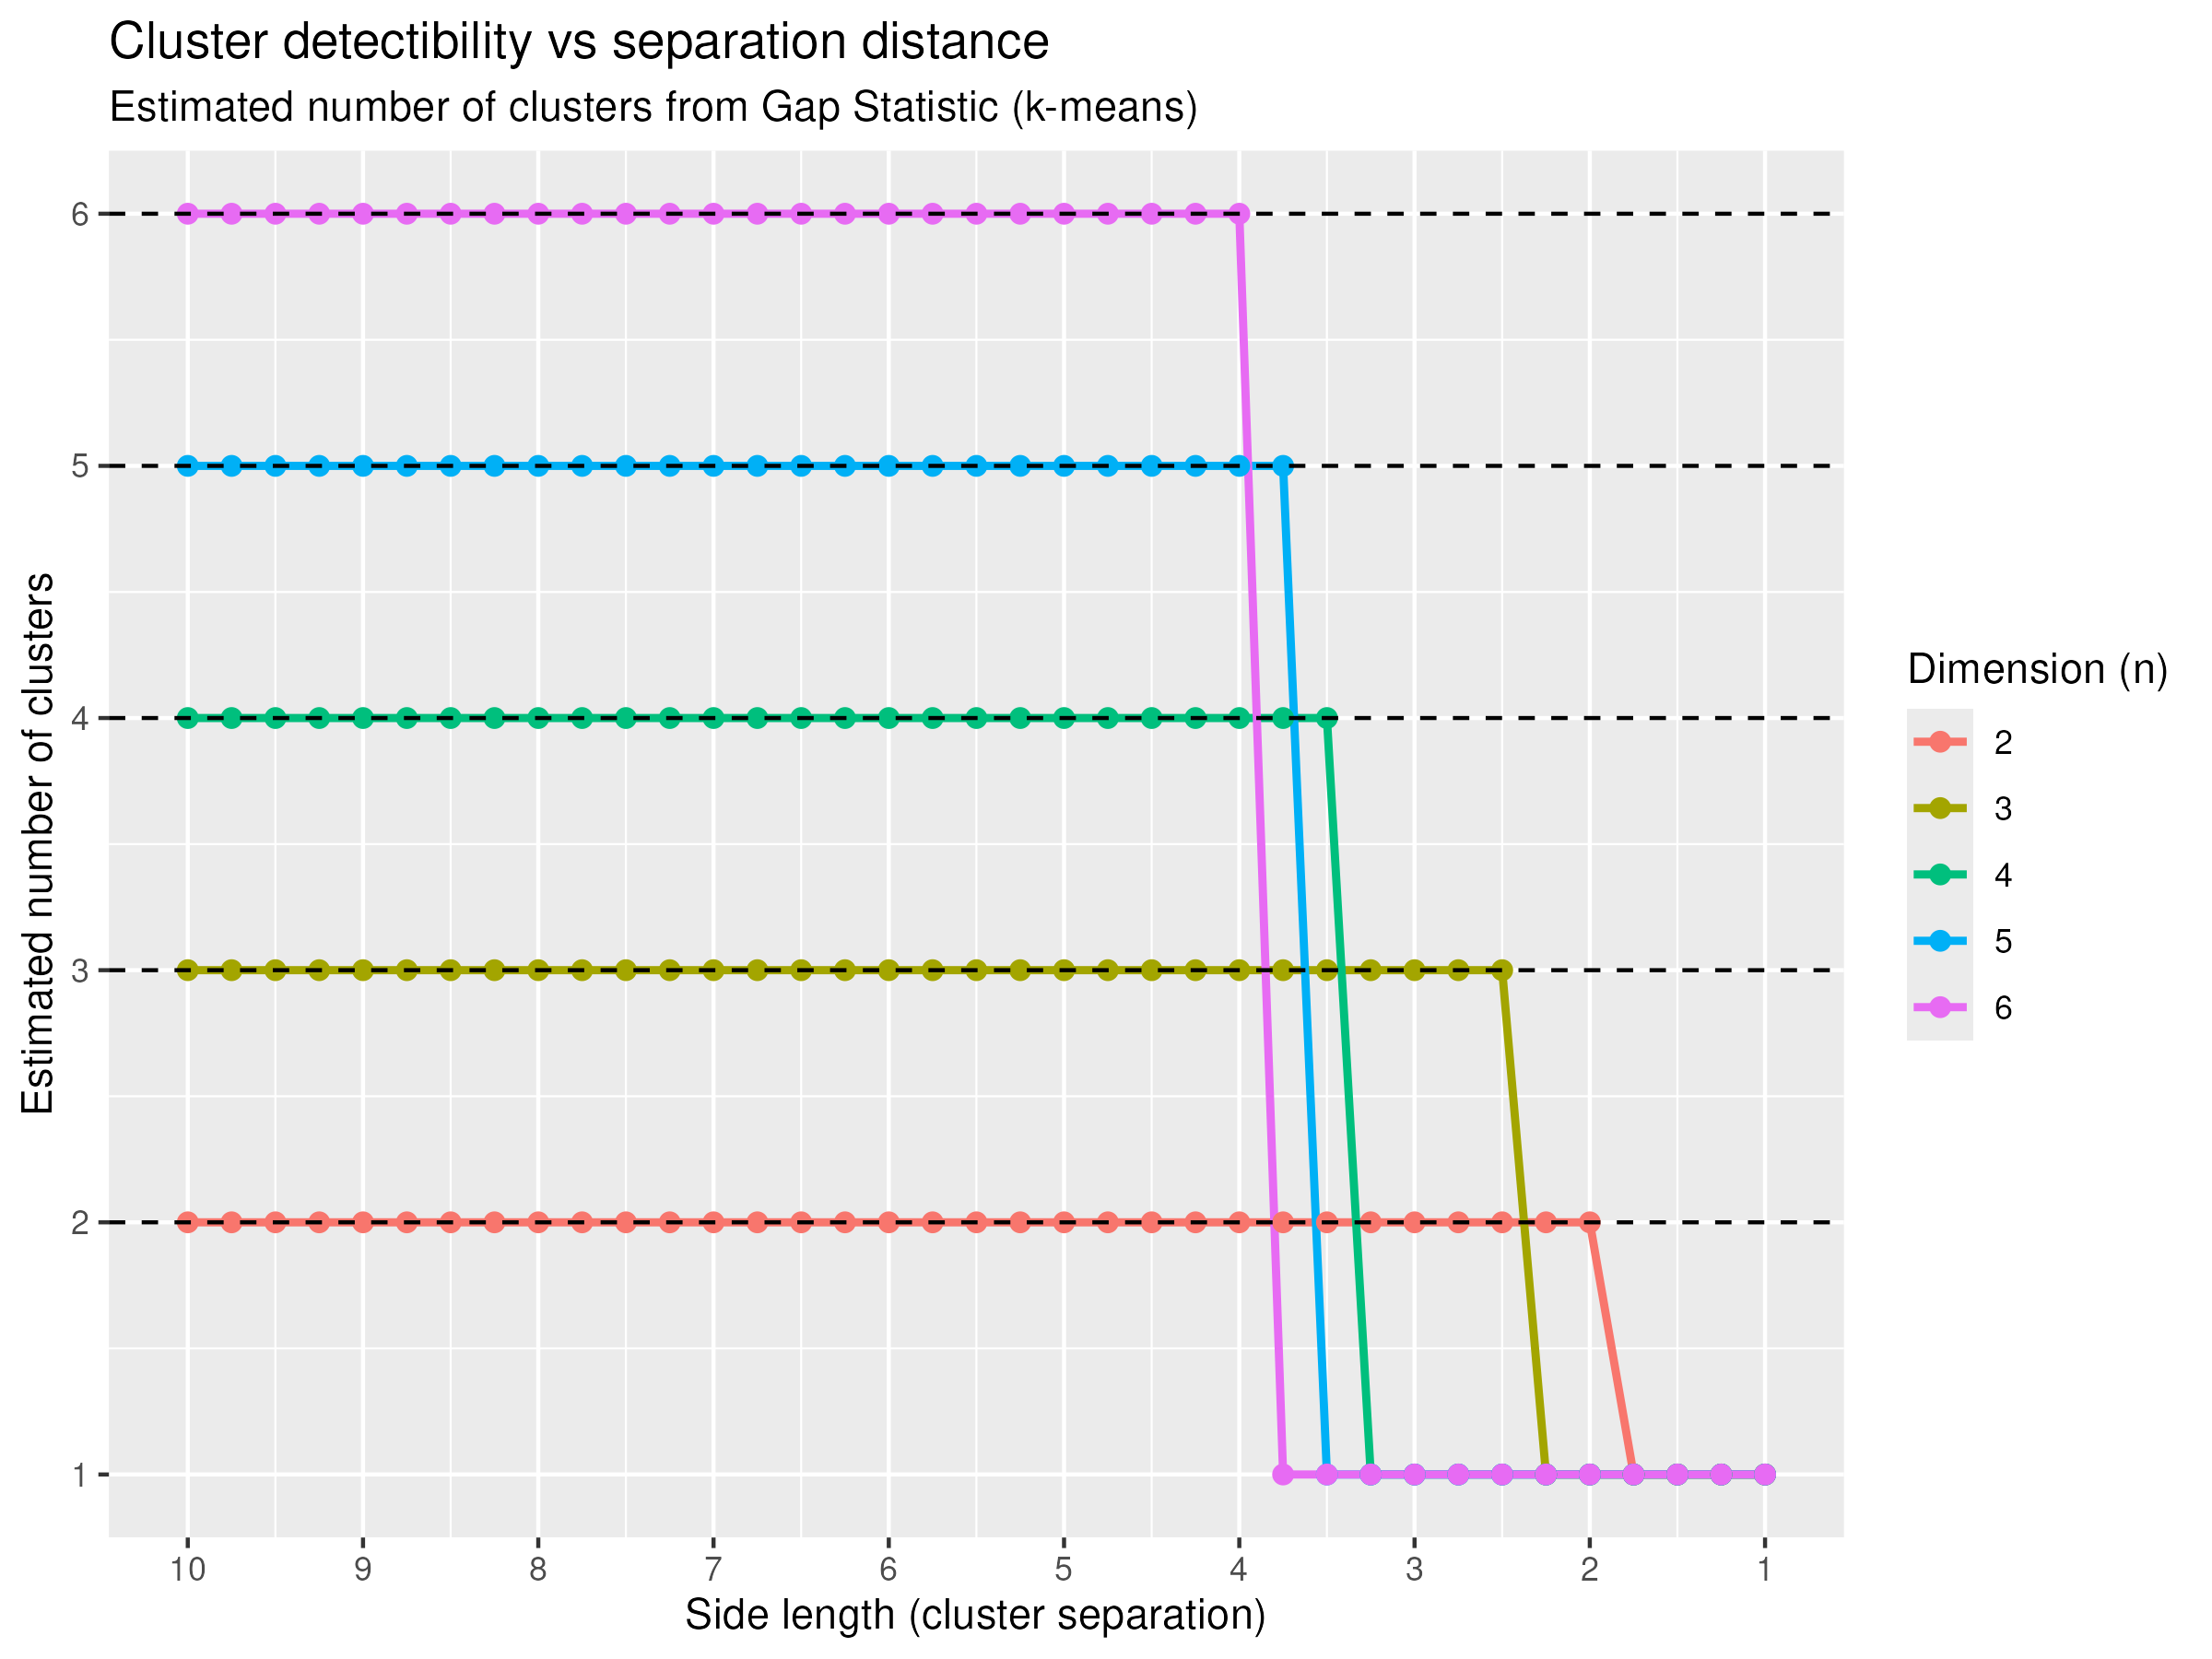
\includegraphics[keepaspectratio,alt={Cluster Detectability with k-Means}]{"figures/cluster_detectability_kmeans.png"}}
\caption{Cluster Detectability with k-Means}
\end{figure}

\section{Task 2: Spectral Clustering on 3D Shell
Data}\label{task-2-spectral-clustering-on-3d-shell-data}

In the second task, I implemented spectral clustering on data arranged
in three-dimensional shells, designed to test whether the algorithm
could distinguish multiple concentric clusters as they were moved closer
together.

Each dataset consisted of four shells with evenly spaced radii between 0
and a set maximum radius, with 100 points per shell. Points were
connected in a similarity graph using an adjacency matrix where
\(A_{ij} = 1\) if the Euclidean distance between points \(i\) and \(j\)
was less than 1 (the fixed distance threshold). However, this setup led
to challenges:

\begin{itemize}
\tightlist
\item
  For larger maximum radii (e.g., 10), the outer shells were too sparse.
  Many points were isolated because no other points were within the
  threshold distance.
\item
  These disconnected nodes caused instability and poor performance in
  spectral clustering and k-means applied to the eigenvector
  representations.
\item
  Increasing the distance threshold connected the graph more fully but
  began to blur boundaries between inner shells, reducing separability.
\end{itemize}

I attempted a modification to the adjacency matrix construction: if a
point had no neighbors within the distance threshold, it was connected
to its three nearest neighbors. This reduced sparsity but did not fix
the core issue. \texttt{clusGap()} still tended to select one cluster
across all configurations.

Because constructing the Laplacian and performing eigen-decomposition
scale approximately with the square of the number of points
(\(O(n^2)\)), increasing the number of points per shell to fix sparsity
quickly became computationally expensive.

In summary, smaller distance thresholds lead to disconnected graphs
preventing meaningful structure in the eigenvector representation, and
larger thresholds can overconnect the graph and inappropriately merge
clusters. Adding more points per shell could help, but with a
substantial computational cost.

The figure below shows the poor detectability behavior using 100 points
per cluster and a distance threshold of 1.

\begin{figure}
\centering
\pandocbounded{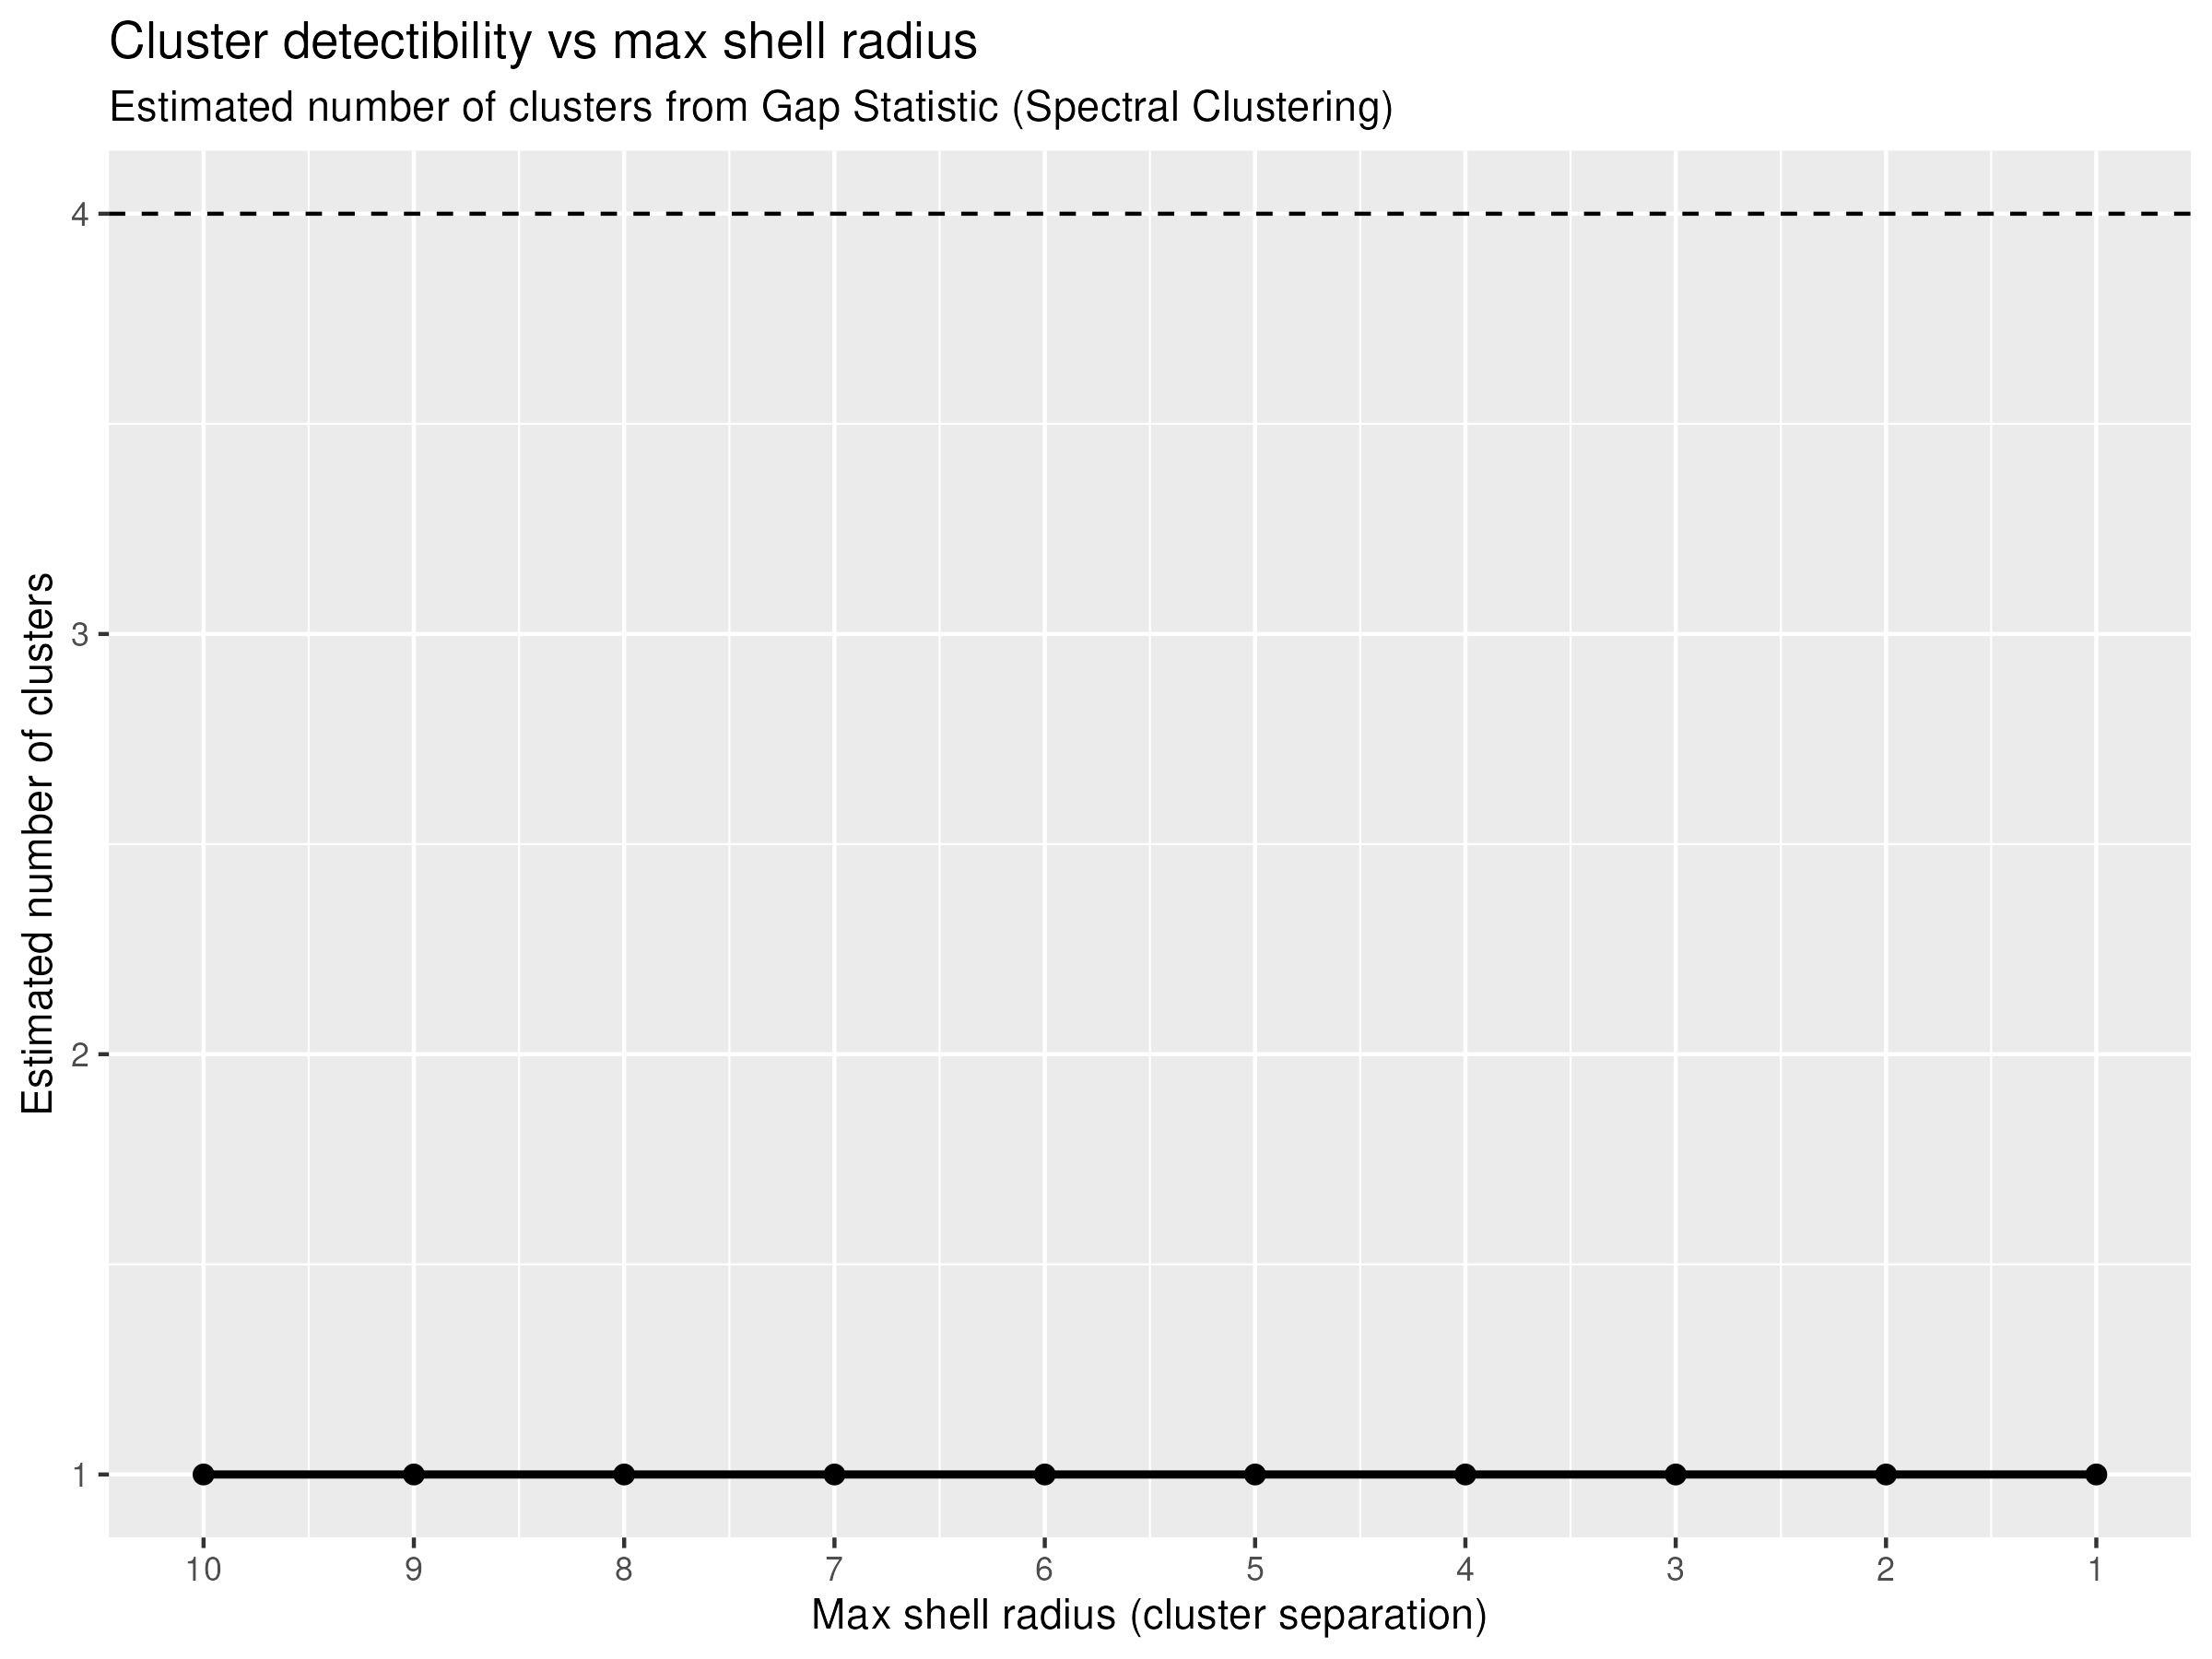
\includegraphics[keepaspectratio,alt={Cluster Detectability with Spectral Clustering}]{figures/cluster_detectability_spec.png}}
\caption{Cluster Detectability with Spectral Clustering}
\end{figure}

\end{document}
